\documentclass{report}

\usepackage{blindtext}
\usepackage{graphicx}
\usepackage{caption}
\usepackage{subcaption}
\usepackage[margin=0.5in]{geometry}

\graphicspath{ {./images/} }

\author{Oskar Mampe: 201368087}
\date{\today}
\title{Convolutional Neural Networks}

\begin{document}
    \maketitle
    \tableofcontents

    \section{Part I: Experimenting with Features}
    Firstly, for my experiments, I have tested various number of layers to see how it affects the performance of the network. I have also decided to validate the performance of different filter size's of the two proceeding convolutional layers. These are the confusion matrices that I have generated for different layers:
    \begin{figure}[h!]
        \centering
        \begin{subfigure}[t]{0.45\textwidth}
            \centering
            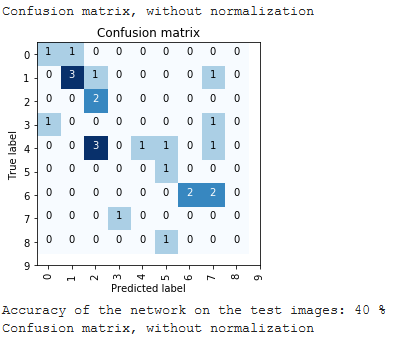
\includegraphics[width=0.5\textwidth]{2_layers}
            \caption{2 Layer Network}
        \end{subfigure}
        \begin{subfigure}[t]{0.45\textwidth}
            \centering
            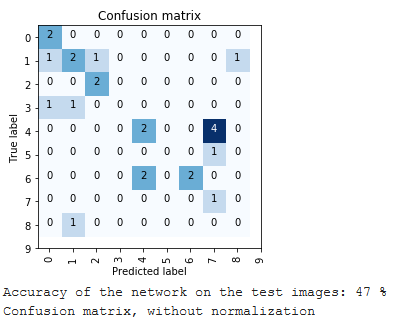
\includegraphics[width=0.5\textwidth]{3_layers}
            \caption{3 Layer Network}
        \end{subfigure}
        \begin{subfigure}[t]{0.45\textwidth}
            \centering
            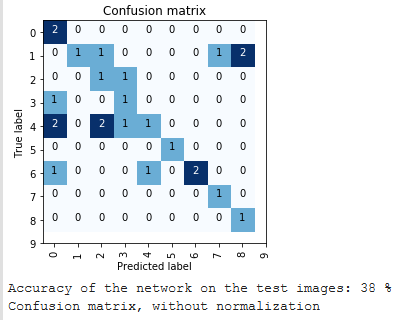
\includegraphics[width=0.5\textwidth]{4_layers}
            \caption{4 Layer Network}
        \end{subfigure}
        \begin{subfigure}[t]{0.45\textwidth}
            \centering
            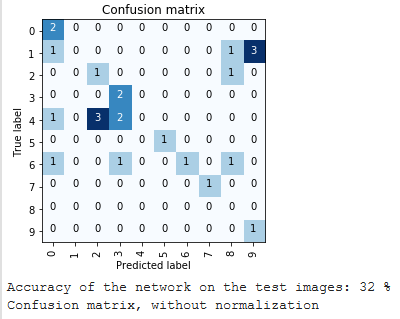
\includegraphics[width=0.5\textwidth]{5_layers}
            \caption{5 Layer Network}
        \end{subfigure}
        \caption{Confusion Matrices for the Different Layers}
    \end{figure}

    As you can see, the layers perform better with a lower number of layers, the sweet spot being around 3.
    \begin{figure}[h!]
        \centering
        \begin{subfigure}[t]{0.45\textwidth}
            \centering
            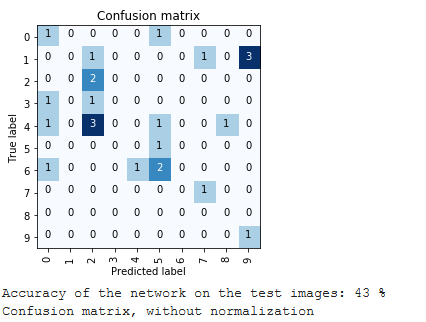
\includegraphics[width=0.5\textwidth]{2_ks}
            \caption{2 Filter Size Network}
        \end{subfigure}
        \begin{subfigure}[t]{0.45\textwidth}
            \centering
            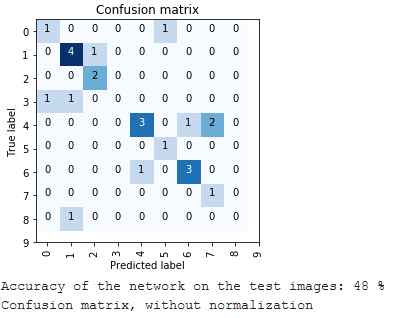
\includegraphics[width=0.5\textwidth]{3_ks}
            \caption{3 Filter Size Network}
        \end{subfigure}
        \begin{subfigure}[t]{0.45\textwidth}
            \centering
            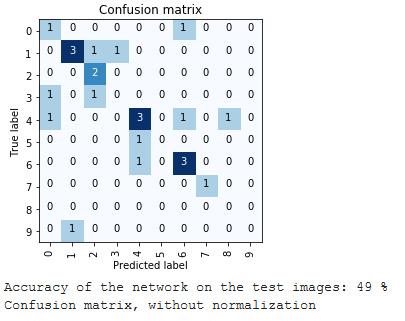
\includegraphics[width=0.5\textwidth]{4_ks}
            \caption{4 Filter Size Network}
        \end{subfigure}
        \begin{subfigure}[t]{0.45\textwidth}
            \centering
            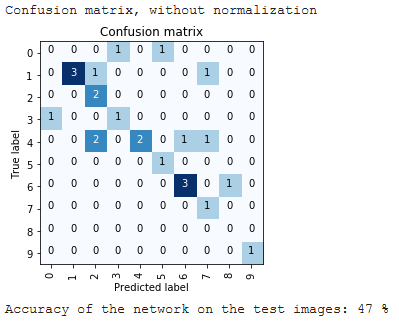
\includegraphics[width=0.5\textwidth]{5_ks}
            \caption{5 Filter Size Network}
        \end{subfigure}
        \caption{Confusion Matrices for the Different Layers}
    \end{figure}


    \section{Part II: Visualising Filters}

    \section{Part III: Visualising Features}

    \section{Part IV: Experimenting with Network}

\end{document}